\begin{figure}[ht]
\centering
\definecolor{convfront}{HTML}{B8CCE4}
\definecolor{convtop}{HTML}{D0DEF0}
\definecolor{convside}{HTML}{8FAEC8}
\definecolor{fcfront}{HTML}{C5D5C5}
\definecolor{fctop}{HTML}{D8E6D8}
\definecolor{fcside}{HTML}{9AB89A}
\definecolor{outfront}{HTML}{D4C5B0}
\definecolor{outtop}{HTML}{E4D8C8}
\definecolor{outside}{HTML}{B8A890}
\resizebox{0.85\textwidth}{!}{%
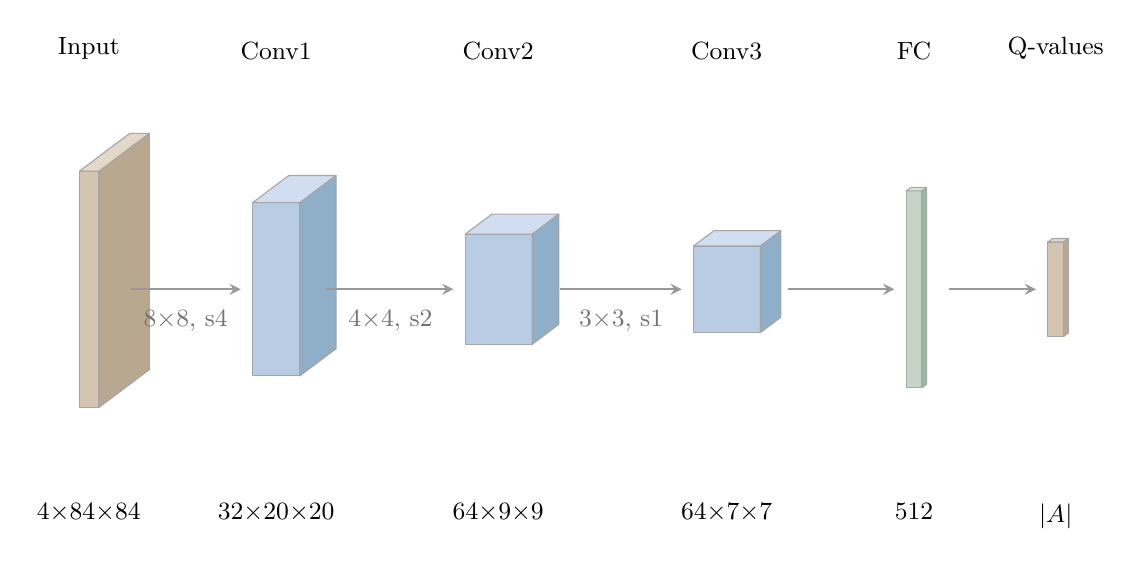
\begin{tikzpicture}[
    x={(1cm,0cm)}, y={(0cm,1cm)}, z={(0.4cm,0.3cm)},
    arr/.style={->, thick, >=stealth, black!40},
    dimlbl/.style={font=\small, anchor=north},
    namelbl/.style={font=\small, anchor=south},
    filtlbl/.style={font=\small, text=black!55, anchor=north}
]

\newcommand{\cuboid}[7]{
    \fill[#5, draw=black!35, line join=round]
        (#1, {-#3/2}, 0) -- ({#1+#2}, {-#3/2}, 0) --
        ({#1+#2}, {#3/2}, 0) -- (#1, {#3/2}, 0) -- cycle;
    \fill[#6, draw=black!35, line join=round]
        (#1, {#3/2}, 0) -- ({#1+#2}, {#3/2}, 0) --
        ({#1+#2}, {#3/2}, #4) -- (#1, {#3/2}, #4) -- cycle;
    \fill[#7, draw=black!35, line join=round]
        ({#1+#2}, {-#3/2}, 0) -- ({#1+#2}, {#3/2}, 0) --
        ({#1+#2}, {#3/2}, #4) -- ({#1+#2}, {-#3/2}, #4) -- cycle;
}

% Baselines
\def\dimY{-2.6}
\def\nameY{2.8}

% Input: 4 x 84 x 84
\cuboid{0.8}{0.25}{3.0}{1.6}{outfront}{outtop}{outside}
\node[namelbl] at (0.92, \nameY, 0) {Input};
\node[dimlbl] at (0.92, \dimY, 0) {4${\times}$84${\times}$84};

% Arrow + label below
\draw[arr] (1.45, 0, 0) -- (2.85, 0, 0);
\node[filtlbl] at (2.15, -0.15, 0) {8${\times}$8, s4};

% Conv1: 32 x 20 x 20
\cuboid{3.0}{0.6}{2.2}{1.15}{convfront}{convtop}{convside}
\node[namelbl] at (3.3, \nameY, 0) {Conv1};
\node[dimlbl] at (3.3, \dimY, 0) {32${\times}$20${\times}$20};

% Arrow + label below
\draw[arr] (3.95, 0, 0) -- (5.55, 0, 0);
\node[filtlbl] at (4.75, -0.15, 0) {4${\times}$4, s2};

% Conv2: 64 x 9 x 9
\cuboid{5.7}{0.85}{1.4}{0.85}{convfront}{convtop}{convside}
\node[namelbl] at (6.12, \nameY, 0) {Conv2};
\node[dimlbl] at (6.12, \dimY, 0) {64${\times}$9${\times}$9};

% Arrow + label below
\draw[arr] (6.9, 0, 0) -- (8.45, 0, 0);
\node[filtlbl] at (7.68, -0.15, 0) {3${\times}$3, s1};

% Conv3: 64 x 7 x 7
\cuboid{8.6}{0.85}{1.1}{0.65}{convfront}{convtop}{convside}
\node[namelbl] at (9.02, \nameY, 0) {Conv3};
\node[dimlbl] at (9.02, \dimY, 0) {64${\times}$7${\times}$7};

% Arrow
\draw[arr] (9.8, 0, 0) -- (11.15, 0, 0);

% FC: 512
\cuboid{11.3}{0.2}{2.5}{0.15}{fcfront}{fctop}{fcside}
\node[namelbl] at (11.4, \nameY, 0) {FC};
\node[dimlbl] at (11.4, \dimY, 0) {512};

% Arrow
\draw[arr] (11.85, 0, 0) -- (12.95, 0, 0);

% Q-values
\cuboid{13.1}{0.2}{1.2}{0.15}{outfront}{outtop}{outside}
\node[namelbl] at (13.2, \nameY, 0) {Q-values};
\node[dimlbl] at (13.2, \dimY, 0) {$|A|$};

\end{tikzpicture}%
}
\caption{Nature CNN architecture. Block height reflects spatial
  dimensions; block depth reflects channel count. All convolutional
  and fully connected layers use ReLU activation.}
\label{fig:nature-cnn}
\end{figure}
